\FloatBarrier
\subsection{Question 6}
We mirror zeros of the transfer function then we apply a moving average controller using \autoref{code:sstr61}. As shown in \autoref{fig:sstr61}, the system remains stable and, when actuated, returns to its equilibrium point at $0$. As shown in \autoref{fig:sstr62}, cummulative loss of the system is bounded.

\begin{code}
	\begin{matlabcode}{firstnumber = 1}
%%  Original unstable system
G_s = 3*(0.4*s-1)*(s-0.8)/((3*s+1)^2*(s-1));

%%  Discretize the system
G_z = c2d(G_s, Ts, 'zoh');
[B, A] = tfdata(G_z, 'v');
B(1) = [];  

%%  Solve Diophantine equation for d = 2 
d = 2;  % d0=1
[F, G] = diophantine(A, C, d);

%%  Define the MA controller 
MA_controller = tf(conv(F,A), B, Ts);

%%  Define the open loop system
G_ol = minreal(G_z * MA_controller);

%%  Closed-loop system
G_cl = feedback(G_ol, 1);

	\end{matlabcode}
	\captionof{listing}{Moving average controller with mirrored zeros}
	\label{code:sstr61}
\end{code}

\begin{figure}
	\centering
	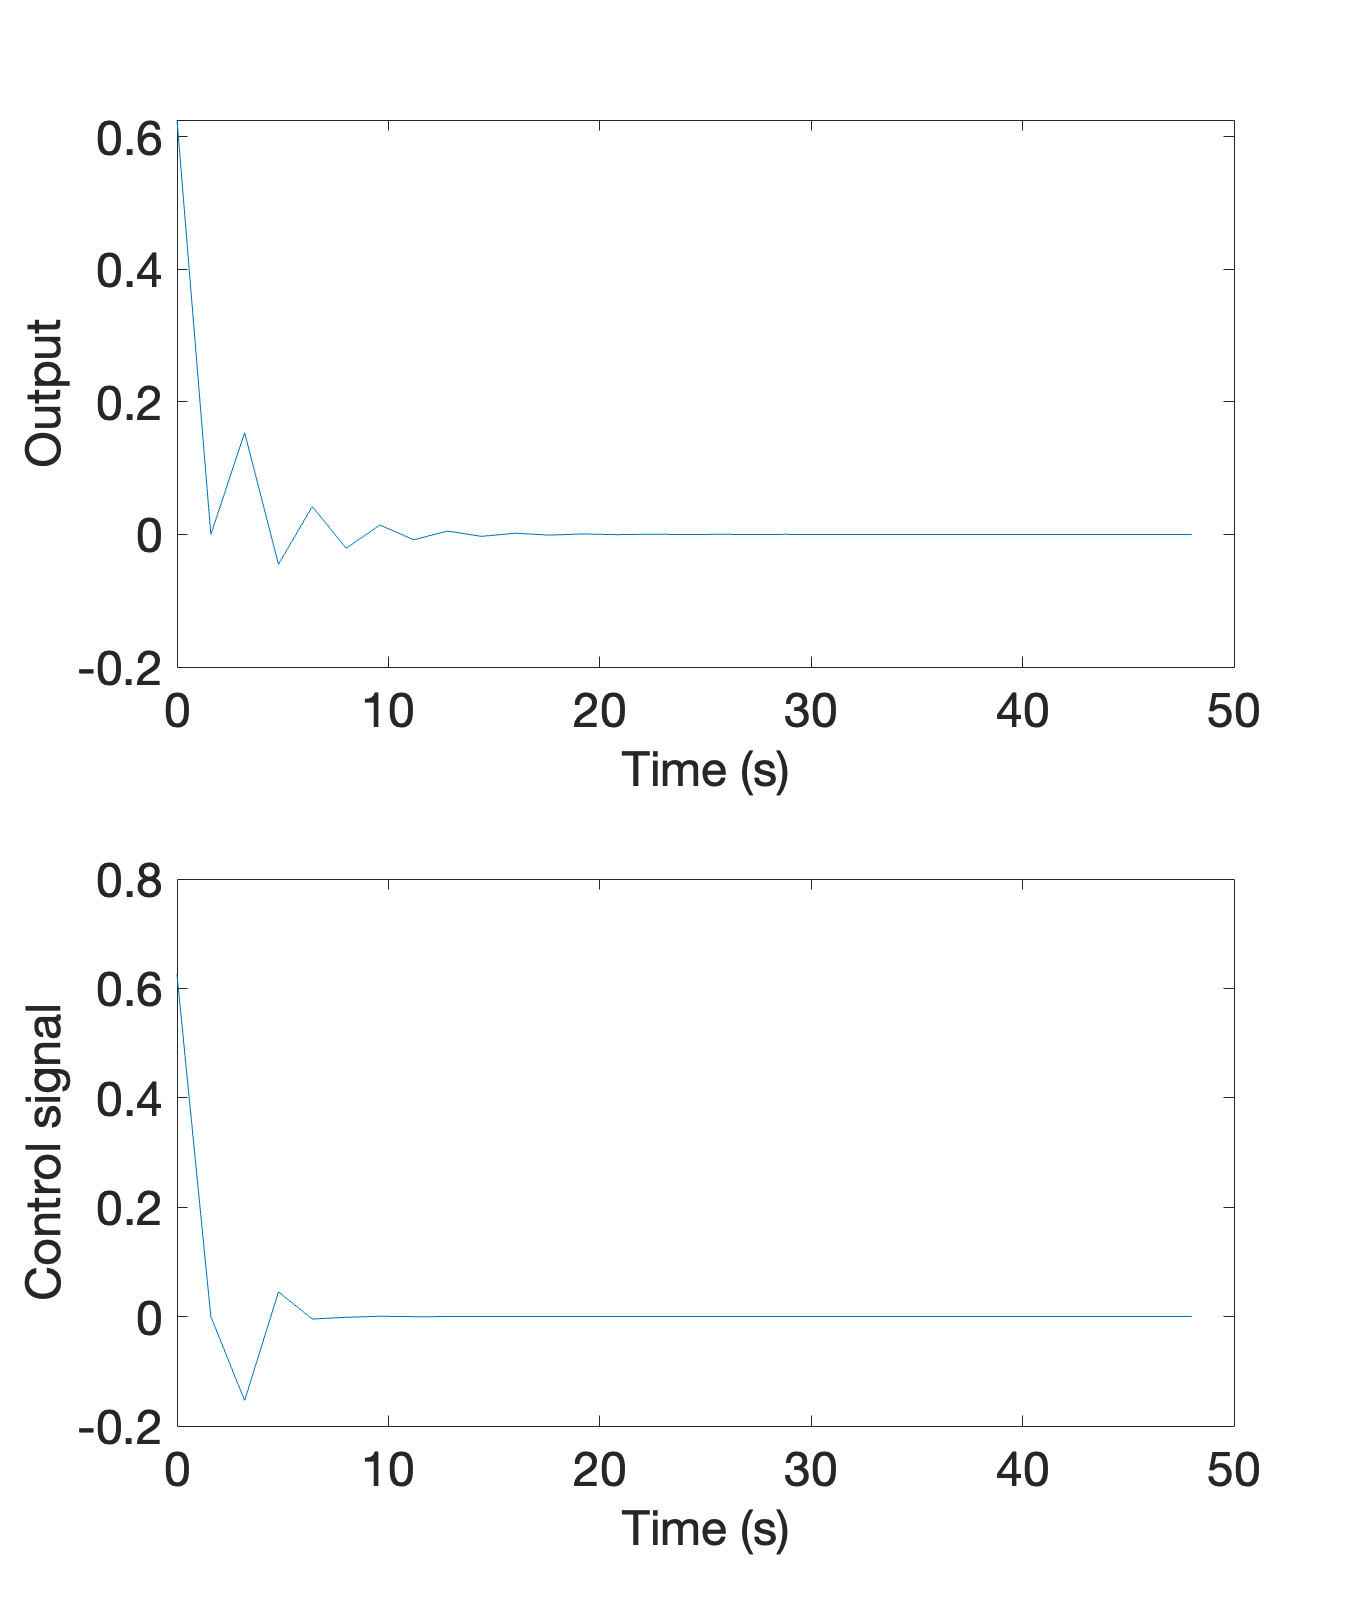
\includegraphics[width=\textwidth]{images/sstr61.png}
	\caption{Output and control of moving average controller with mirrored zeros}
	\label{fig:sstr61}
\end{figure}

\begin{figure}
	\centering
	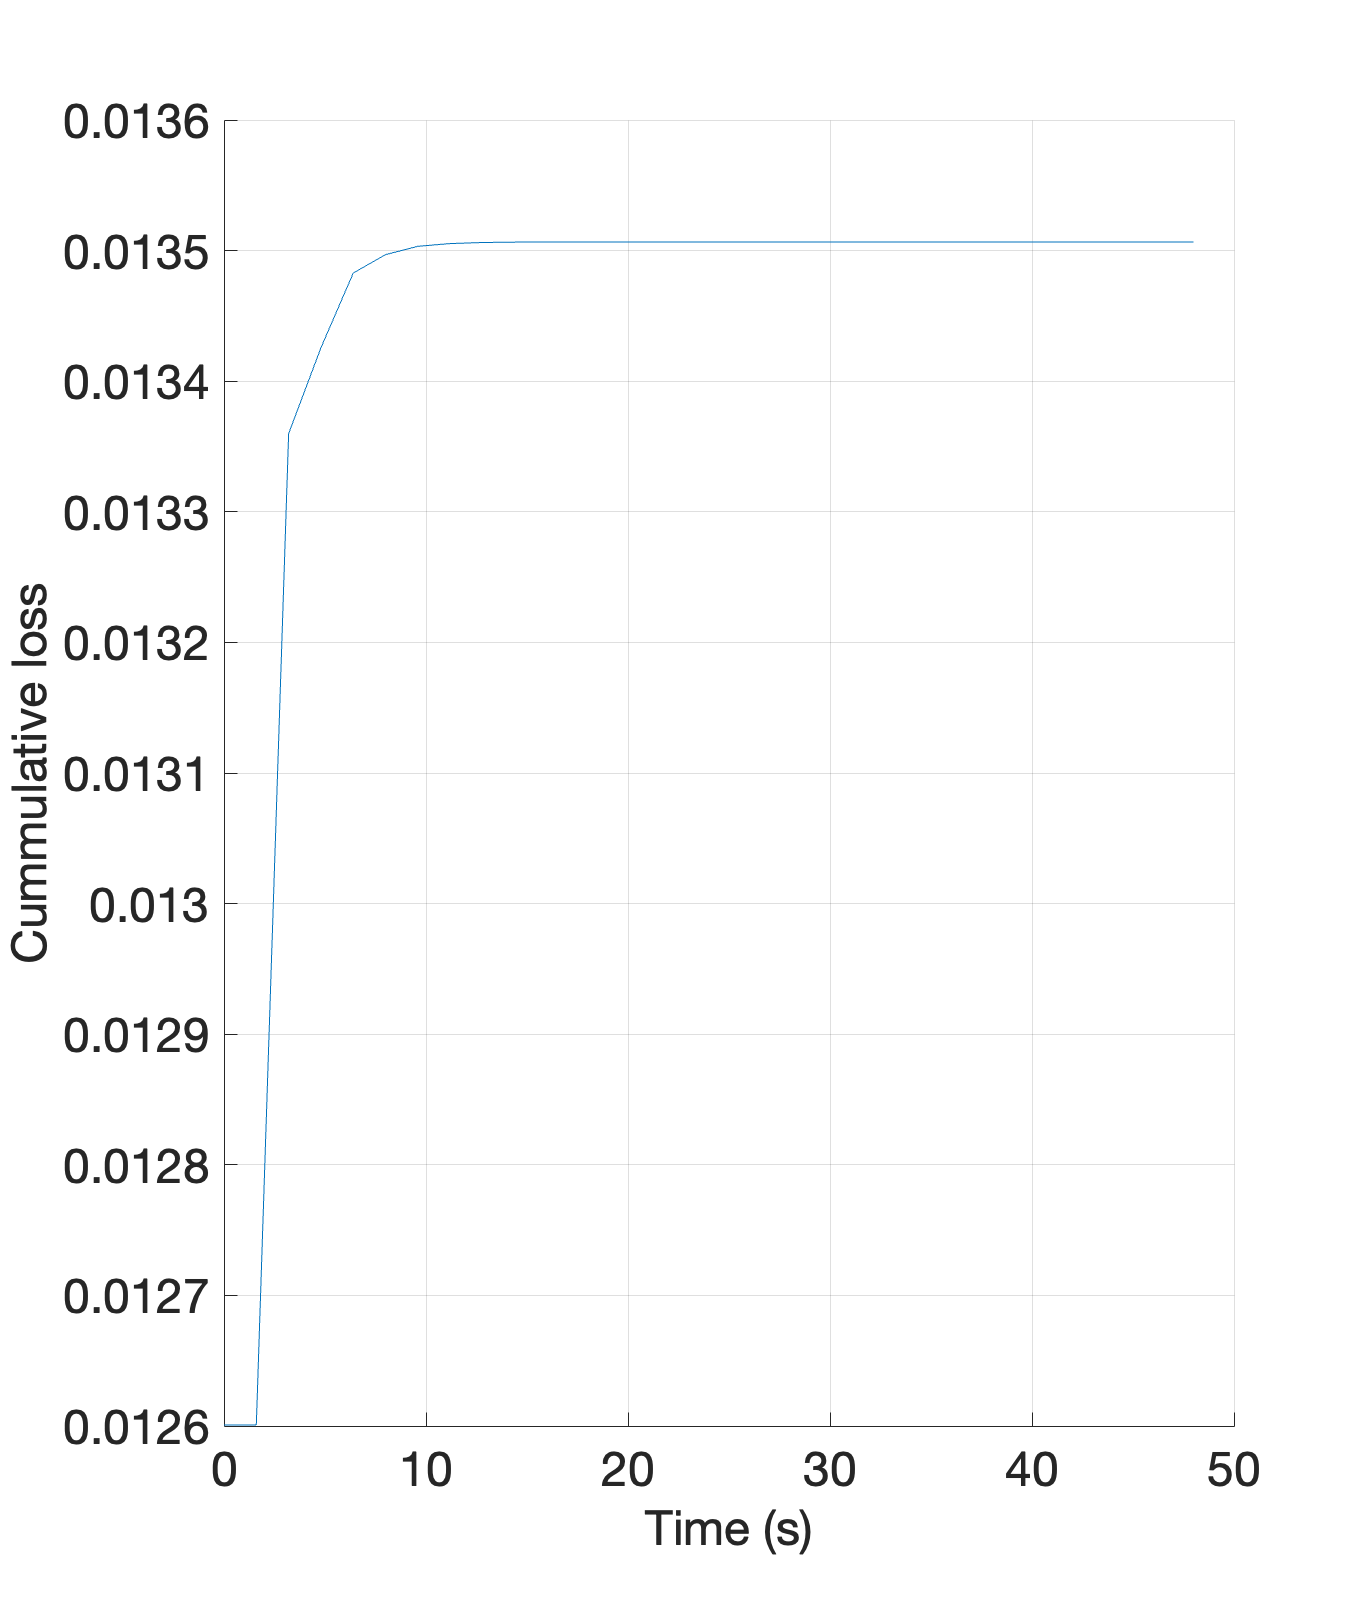
\includegraphics[width=\textwidth]{images/sstr62.png}
	\caption{Cummulative loss of moving average controller with mirrored zeros}
	\label{fig:sstr62}
\end{figure}



\noindent The code for this section is available at \lstinline|assignment3/SSTR/SSTR_6.m|. 

